\documentclass[12pt,twoside,letterpaper]{article}
%NOTE: This report format is 

\newcommand{\reporttitle}{Taipei 101 Tower Analysis}
\newcommand{\reportauthorOne}{John Tattersall}
\newcommand{\cidOne}{20653035}
\newcommand{\reportauthorTwo}{David Beckett}
\newcommand{\cidTwo}{20655588}
\newcommand{\reporttype}{Coursework}
\bibliographystyle{plain}

% include files that load packages and define macros
%%%%%%%%%%%%%%%%%%%%%%%%%%%%%%%%%%%%%%%%%
% University Assignment Title Page 
% LaTeX Template
% Version 1.0 (27/12/12)
%
% This template has been downloaded from:
% http://www.LaTeXTemplates.com
%
% Original author:
% WikiBooks (http://en.wikibooks.org/wiki/LaTeX/Title_Creation)
%
% License:
% CC BY-NC-SA 3.0 (http://creativecommons.org/licenses/by-nc-sa/3.0/)
% 
% Instructions for using this template:
% This title page is capable of being compiled as is. This is not useful for 
% including it in another document. To do this, you have two options: 
%
% 1) Copy/paste everything between \begin{document} and \end{document} 
% starting at \begin{titlepage} and paste this into another LaTeX file where you 
% want your title page.
% OR
% 2) Remove everything outside the \begin{titlepage} and \end{titlepage} and 
% move this file to the same directory as the LaTeX file you wish to add it to. 
% Then add \input{./title_page_1.tex} to your LaTeX file where you want your
% title page.
%
%----------------------------------------------------------------------------------------
%	PACKAGES AND OTHER DOCUMENT CONFIGURATIONS
%----------------------------------------------------------------------------------------
\usepackage{ifxetex}
\usepackage{textpos}
\usepackage{natbib}
\usepackage{kpfonts}
\usepackage[letterpaper,hmargin=2.8cm,vmargin=2.0cm,includeheadfoot]{geometry}
\usepackage{ifxetex}
\usepackage{stackengine}
\usepackage{tabularx,longtable,multirow,subfigure,caption}%hangcaption
\usepackage{fncylab} %formatting of labels
\usepackage{fancyhdr}
\usepackage{color}
\usepackage[tight,ugly]{units}
\usepackage{url}
\usepackage{float}
\usepackage[english]{babel}
\usepackage{amsmath}
\usepackage{graphicx}
\usepackage[colorinlistoftodos]{todonotes}
\usepackage{dsfont}
\usepackage{epstopdf} % automatically replace .eps with .pdf in graphics
\usepackage{natbib}
\usepackage{backref}
\usepackage{array}
\usepackage{latexsym}
\usepackage{etoolbox}

\usepackage{enumerate} % for numbering with [a)] format 



\ifxetex
\usepackage{fontspec}
\setmainfont[Scale=.8]{OpenDyslexic-Regular}
\else
\usepackage[pdftex,pagebackref,hypertexnames=false,colorlinks]{hyperref} % provide links in pdf
\hypersetup{pdftitle={},
  pdfsubject={}, 
  pdfauthor={\reportauthorOne},
  pdfkeywords={}, 
  pdfstartview=FitH,
  pdfpagemode={UseOutlines},% None, FullScreen, UseOutlines
  bookmarksnumbered=true, bookmarksopen=true, colorlinks,
    citecolor=black,%
    filecolor=black,%
    linkcolor=black,%
    urlcolor=black}
\usepackage[all]{hypcap}
\fi

\usepackage{tcolorbox}

% various theorems
\usepackage{ntheorem}
\theoremstyle{break}
\newtheorem{lemma}{Lemma}
\newtheorem{theorem}{Theorem}
\newtheorem{remark}{Remark}
\newtheorem{definition}{Definition}
\newtheorem{proof}{Proof}

% example-environment
\newenvironment{example}[1][]
{ 
\vspace{4mm}
\noindent\makebox[\linewidth]{\rule{\hsize}{1.5pt}}
\textbf{Example #1}\\
}
{ 
\noindent\newline\makebox[\linewidth]{\rule{\hsize}{1.0pt}}
}



%\renewcommand{\rmdefault}{pplx} % Palatino
% \renewcommand{\rmdefault}{put} % Utopia

\ifxetex
\else
\renewcommand*{\rmdefault}{bch} % Charter
\renewcommand*{\ttdefault}{cmtt} % Computer Modern Typewriter
%\renewcommand*{\rmdefault}{phv} % Helvetica
%\renewcommand*{\rmdefault}{iwona} % Avant Garde
\fi

\setlength{\parindent}{0em}  % indentation of paragraph

\setlength{\headheight}{14.5pt}
\pagestyle{fancy}
\fancyfoot[ER,OL]{\thepage}%Page no. in the left on
                                %odd pages and on right on even pages
\fancyfoot[OC,EC]{\sffamily }
\renewcommand{\headrulewidth}{0.1pt}
\renewcommand{\footrulewidth}{0.1pt}
\captionsetup{margin=10pt,font=small,labelfont=bf}


%--- chapter heading

\def\@makechapterhead#1{%
  \vspace*{10\p@}%
  {\parindent \z@ \raggedright %\sffamily
        %{\Large \MakeUppercase{\@chapapp} \space \thechapter}
        %\\
        %\hrulefill
        %\par\nobreak
        %\vskip 10\p@
    \interlinepenalty\@M
    \Huge \bfseries 
    \thechapter \space\space #1\par\nobreak
    \vskip 30\p@
  }}

%---chapter heading for \chapter*  
\def\@makeschapterhead#1{%
  \vspace*{10\p@}%
  {\parindent \z@ \raggedright
    \sffamily
    \interlinepenalty\@M
    \Huge \bfseries  
    #1\par\nobreak
    \vskip 30\p@
  }}
  



% %%%%%%%%%%%%% boxit
\def\Beginboxit
   {\par
    \vbox\bgroup
	   \hrule
	   \hbox\bgroup
		  \vrule \kern1.2pt %
		  \vbox\bgroup\kern1.2pt
   }

\def\Endboxit{%
			      \kern1.2pt
		       \egroup
		  \kern1.2pt\vrule
		\egroup
	   \hrule
	 \egroup
   }	

\newenvironment{boxit}{\Beginboxit}{\Endboxit}
\newenvironment{boxit*}{\Beginboxit\hbox to\hsize{}}{\Endboxit}



\allowdisplaybreaks

\makeatletter
\newcounter{elimination@steps}
\newcolumntype{R}[1]{>{\raggedleft\arraybackslash$}p{#1}<{$}}
\def\elimination@num@rights{}
\def\elimination@num@variables{}
\def\elimination@col@width{}
\newenvironment{elimination}[4][0]
{
    \setcounter{elimination@steps}{0}
    \def\elimination@num@rights{#1}
    \def\elimination@num@variables{#2}
    \def\elimination@col@width{#3}
    \renewcommand{\arraystretch}{#4}
    \start@align\@ne\st@rredtrue\m@ne
}
{
    \endalign
    \ignorespacesafterend
}
\newcommand{\eliminationstep}[2]
{
    \ifnum\value{elimination@steps}>0\leadsto\quad\fi
    \left[
        \ifnum\elimination@num@rights>0
            \begin{array}
            {@{}*{\elimination@num@variables}{R{\elimination@col@width}}
            |@{}*{\elimination@num@rights}{R{\elimination@col@width}}}
        \else
            \begin{array}
            {@{}*{\elimination@num@variables}{R{\elimination@col@width}}}
        \fi
            #1
        \end{array}
    \right]
    & 
    \begin{array}{l}
        #2
    \end{array}
    &%                                    moved second & here
    \addtocounter{elimination@steps}{1}
}
\makeatother

%% Fast macro for column vectors
\makeatletter  
\def\colvec#1{\expandafter\colvec@i#1,,,,,,,,,\@nil}
\def\colvec@i#1,#2,#3,#4,#5,#6,#7,#8,#9\@nil{% 
  \ifx$#2$ \begin{bmatrix}#1\end{bmatrix} \else
    \ifx$#3$ \begin{bmatrix}#1\\#2\end{bmatrix} \else
      \ifx$#4$ \begin{bmatrix}#1\\#2\\#3\end{bmatrix}\else
        \ifx$#5$ \begin{bmatrix}#1\\#2\\#3\\#4\end{bmatrix}\else
          \ifx$#6$ \begin{bmatrix}#1\\#2\\#3\\#4\\#5\end{bmatrix}\else
            \ifx$#7$ \begin{bmatrix}#1\\#2\\#3\\#4\\#5\\#6\end{bmatrix}\else
              \ifx$#8$ \begin{bmatrix}#1\\#2\\#3\\#4\\#5\\#6\\#7\end{bmatrix}\else
                 \PackageError{Column Vector}{The vector you tried to write is too big, use bmatrix instead}{Try using the bmatrix environment}
              \fi
            \fi
          \fi
        \fi
      \fi
    \fi
  \fi 
}  
\makeatother

\robustify{\colvec}

%%% Local Variables: 
%%% mode: latex
%%% TeX-master: "notes"
%%% End: 
 % various packages needed for maths etc.
% quick way of adding a figure
\newcommand{\fig}[3]{
 \begin{center}
 \scalebox{#3}{\includegraphics[#2]{#1}}
 \end{center}
}

%\newcommand*{\point}[1]{\vec{\mkern0mu#1}}
\newcommand{\ci}[0]{\perp\!\!\!\!\!\perp} % conditional independence
\newcommand{\point}[1]{{#1}} % points 
\renewcommand{\vec}[1]{{\boldsymbol{{#1}}}} % vector
\newcommand{\mat}[1]{{\boldsymbol{{#1}}}} % matrix
\newcommand{\R}[0]{\mathds{R}} % real numbers
\newcommand{\Z}[0]{\mathds{Z}} % integers
\newcommand{\N}[0]{\mathds{N}} % natural numbers
\newcommand{\nat}[0]{\mathds{N}} % natural numbers
\newcommand{\Q}[0]{\mathds{Q}} % rational numbers
\ifxetex
\newcommand{\C}[0]{\mathds{C}} % complex numbers
\else
\newcommand{\C}[0]{\mathds{C}} % complex numbers
\fi
\newcommand{\tr}[0]{\text{tr}} % trace
\renewcommand{\d}[0]{\mathrm{d}} % total derivative
\newcommand{\inv}{^{-1}} % inverse
\newcommand{\id}{\mathrm{id}} % identity mapping
\renewcommand{\dim}{\mathrm{dim}} % dimension
\newcommand{\rank}[0]{\mathrm{rk}} % rank
\newcommand{\determ}[1]{\mathrm{det}(#1)} % determinant
\newcommand{\scp}[2]{\langle #1 , #2 \rangle}
\newcommand{\kernel}[0]{\mathrm{ker}} % kernel/nullspace
\newcommand{\img}[0]{\mathrm{Im}} % image
\newcommand{\idx}[1]{{(#1)}}
\DeclareMathOperator*{\diag}{diag}
\newcommand{\E}{\mathds{E}} % expectation
\newcommand{\var}{\mathds{V}} % variance
\newcommand{\gauss}[2]{\mathcal{N}\big(#1,\,#2\big)} % gaussian distribution N(.,.)
\newcommand{\gaussx}[3]{\mathcal{N}\big(#1\,|\,#2,\,#3\big)} % gaussian distribution N(.|.,.)
\newcommand{\gaussBig}[2]{\mathcal{N}\left(#1,\,#2\right)} % see above, but with brackets that adjust to the height of the arguments
\newcommand{\gaussxBig}[3]{\mathcal{N}\left(#1\,|\,#2,\,#3\right)} % see above, but with brackets that adjust to the height of the arguments
\DeclareMathOperator{\cov}{Cov} % covariance (matrix) 
\ifxetex
\renewcommand{\T}[0]{^\top} % transpose
\else
\newcommand{\T}[0]{^\top}
\fi
% matrix determinant
\newcommand{\matdet}[1]{
\left|
\begin{matrix}
#1
\end{matrix}
\right|
}



%%% various color definitions
\definecolor{darkgreen}{rgb}{0,0.6,0}

\newcommand{\blue}[1]{{\color{blue}#1}}
\newcommand{\red}[1]{{\color{red}#1}}
\newcommand{\green}[1]{{\color{darkgreen}#1}}
\newcommand{\orange}[1]{{\color{orange}#1}}
\newcommand{\magenta}[1]{{\color{magenta}#1}}
\newcommand{\cyan}[1]{{\color{cyan}#1}}


% redefine emph
\renewcommand{\emph}[1]{\blue{\bf{#1}}}

% place a colored box around a character
\gdef\colchar#1#2{%
  \tikz[baseline]{%
  \node[anchor=base,inner sep=2pt,outer sep=0pt,fill = #2!20] {#1};
    }%
}%
 % short-hand notation and macros


%%%%%%%%%%%%%%%%%%%%%%%%%%%%

\begin{document}
% front page
% Last modification: 2016-09-29 (Marc Deisenroth)
% Modification for UW: 2017-05-22 (jphickey)
\begin{titlepage}

\newcommand{\HRule}{\rule{\linewidth}{0.5mm}} % Defines a new command for the horizontal lines, change thickness here


%----------------------------------------------------------------------------------------
%	LOGO SECTION
%----------------------------------------------------------------------------------------



\begin{center} % Center remainder of the page

%----------------------------------------------------------------------------------------
%	HEADING SECTIONS
%----------------------------------------------------------------------------------------


\includegraphics[width = 10cm]{./figures/uw}\\[1.5cm] 
\textbf{\textsc{\Large ME303 - Advanced Engineering Mathematics}}\\[1.0cm] 
\textsc{\Large University of Waterloo}\\[0.5cm] 
\textsc{\large Department of Mechanical and Mechatronics Engineering}\\[0.95cm] 

%----------------------------------------------------------------------------------------
%	TITLE SECTION
%----------------------------------------------------------------------------------------

\HRule \\[0.4cm]
{ \huge \bfseries \reporttitle}\\ % Title of your document
\HRule \\[1.5cm]
\end{center}
%----------------------------------------------------------------------------------------
%	AUTHOR SECTION
%----------------------------------------------------------------------------------------

%\begin{minipage}{0.4\hsize}
\begin{flushleft} \large
\textit{Authors:}\\
\reportauthorOne~(ID: \cidOne)\\ % Your name
\reportauthorTwo~(ID: \cidTwo) % Your name
\end{flushleft}
\vspace{4cm}
\makeatletter
Date: \@date 

\vfill % Fill the rest of the page with whitespace



\makeatother


\end{titlepage}


\pagestyle{plain}

%%%%%%%%%%%%%%%%%%%%%%%%%%% table of content
%If a table of content is needed, simply uncomment the following lines
%\tableofcontents
\newpage
%%%%%%%%%%%%%%%%%%%%%%%%%%%% Main document
\section*{Summary of the Problem}
The Taipei 101 tower was built in 2004 and is known for having the largest mass damper system in the world[4]. A mass damper system makes the horizontal oscillations of a system caused by external forces approach zero at a much faster rate than if it were left alone to sway. In this case the external forces on the tower are winds and ground tremors that can be quite strong if caused by a typhoon or earthquake. To counteract this, a giant mass is hung by cables 12.8m cables from the 91st floor of the building acting like a giant pendulum(Figure 1)[1]. The tuned mass damper (TMD) system  is tuned to the resonant frequency of the building, so when the building bends, the mass smoothly brings it back to equilibrium without causing any discomfort to the residents of the building.

\begin{figure}[h!]
\centering
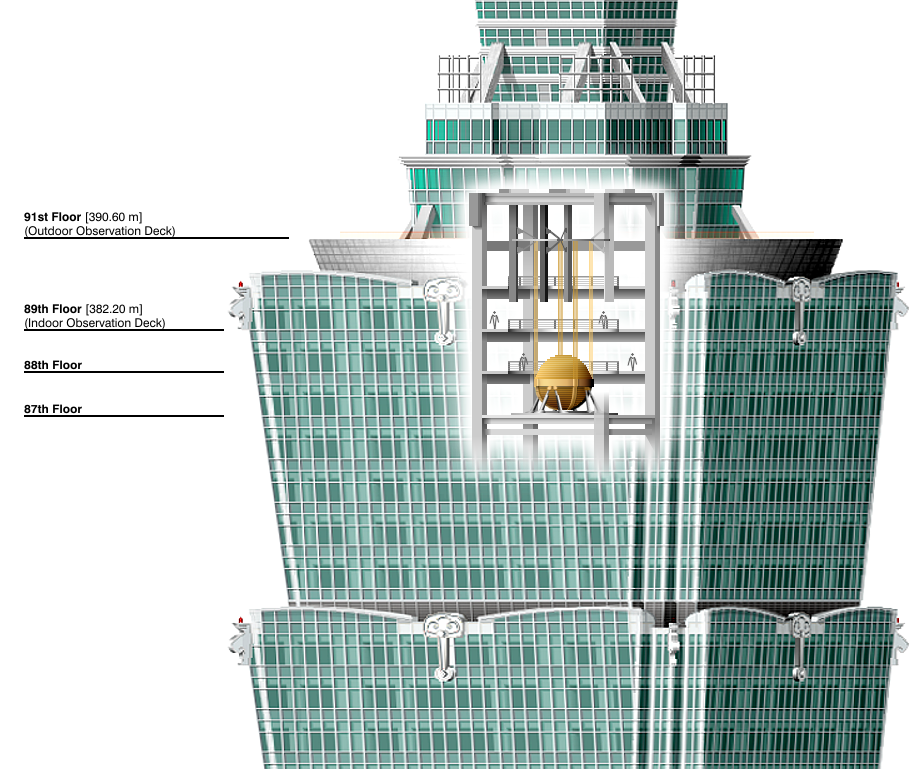
\includegraphics[width=0.45\textwidth]{figures/Taipei101.png} 
\caption{The setup of the Tuned Mass Damper in the Taipei 101 tower}
\label{tower}
\end{figure}

The tower system can be modeled as a single degree of freedom double mass system, with the mass of the building and the mass of the TMD being separate components as modeled in Figure 2.  

\begin{figure}[h!]
\centering
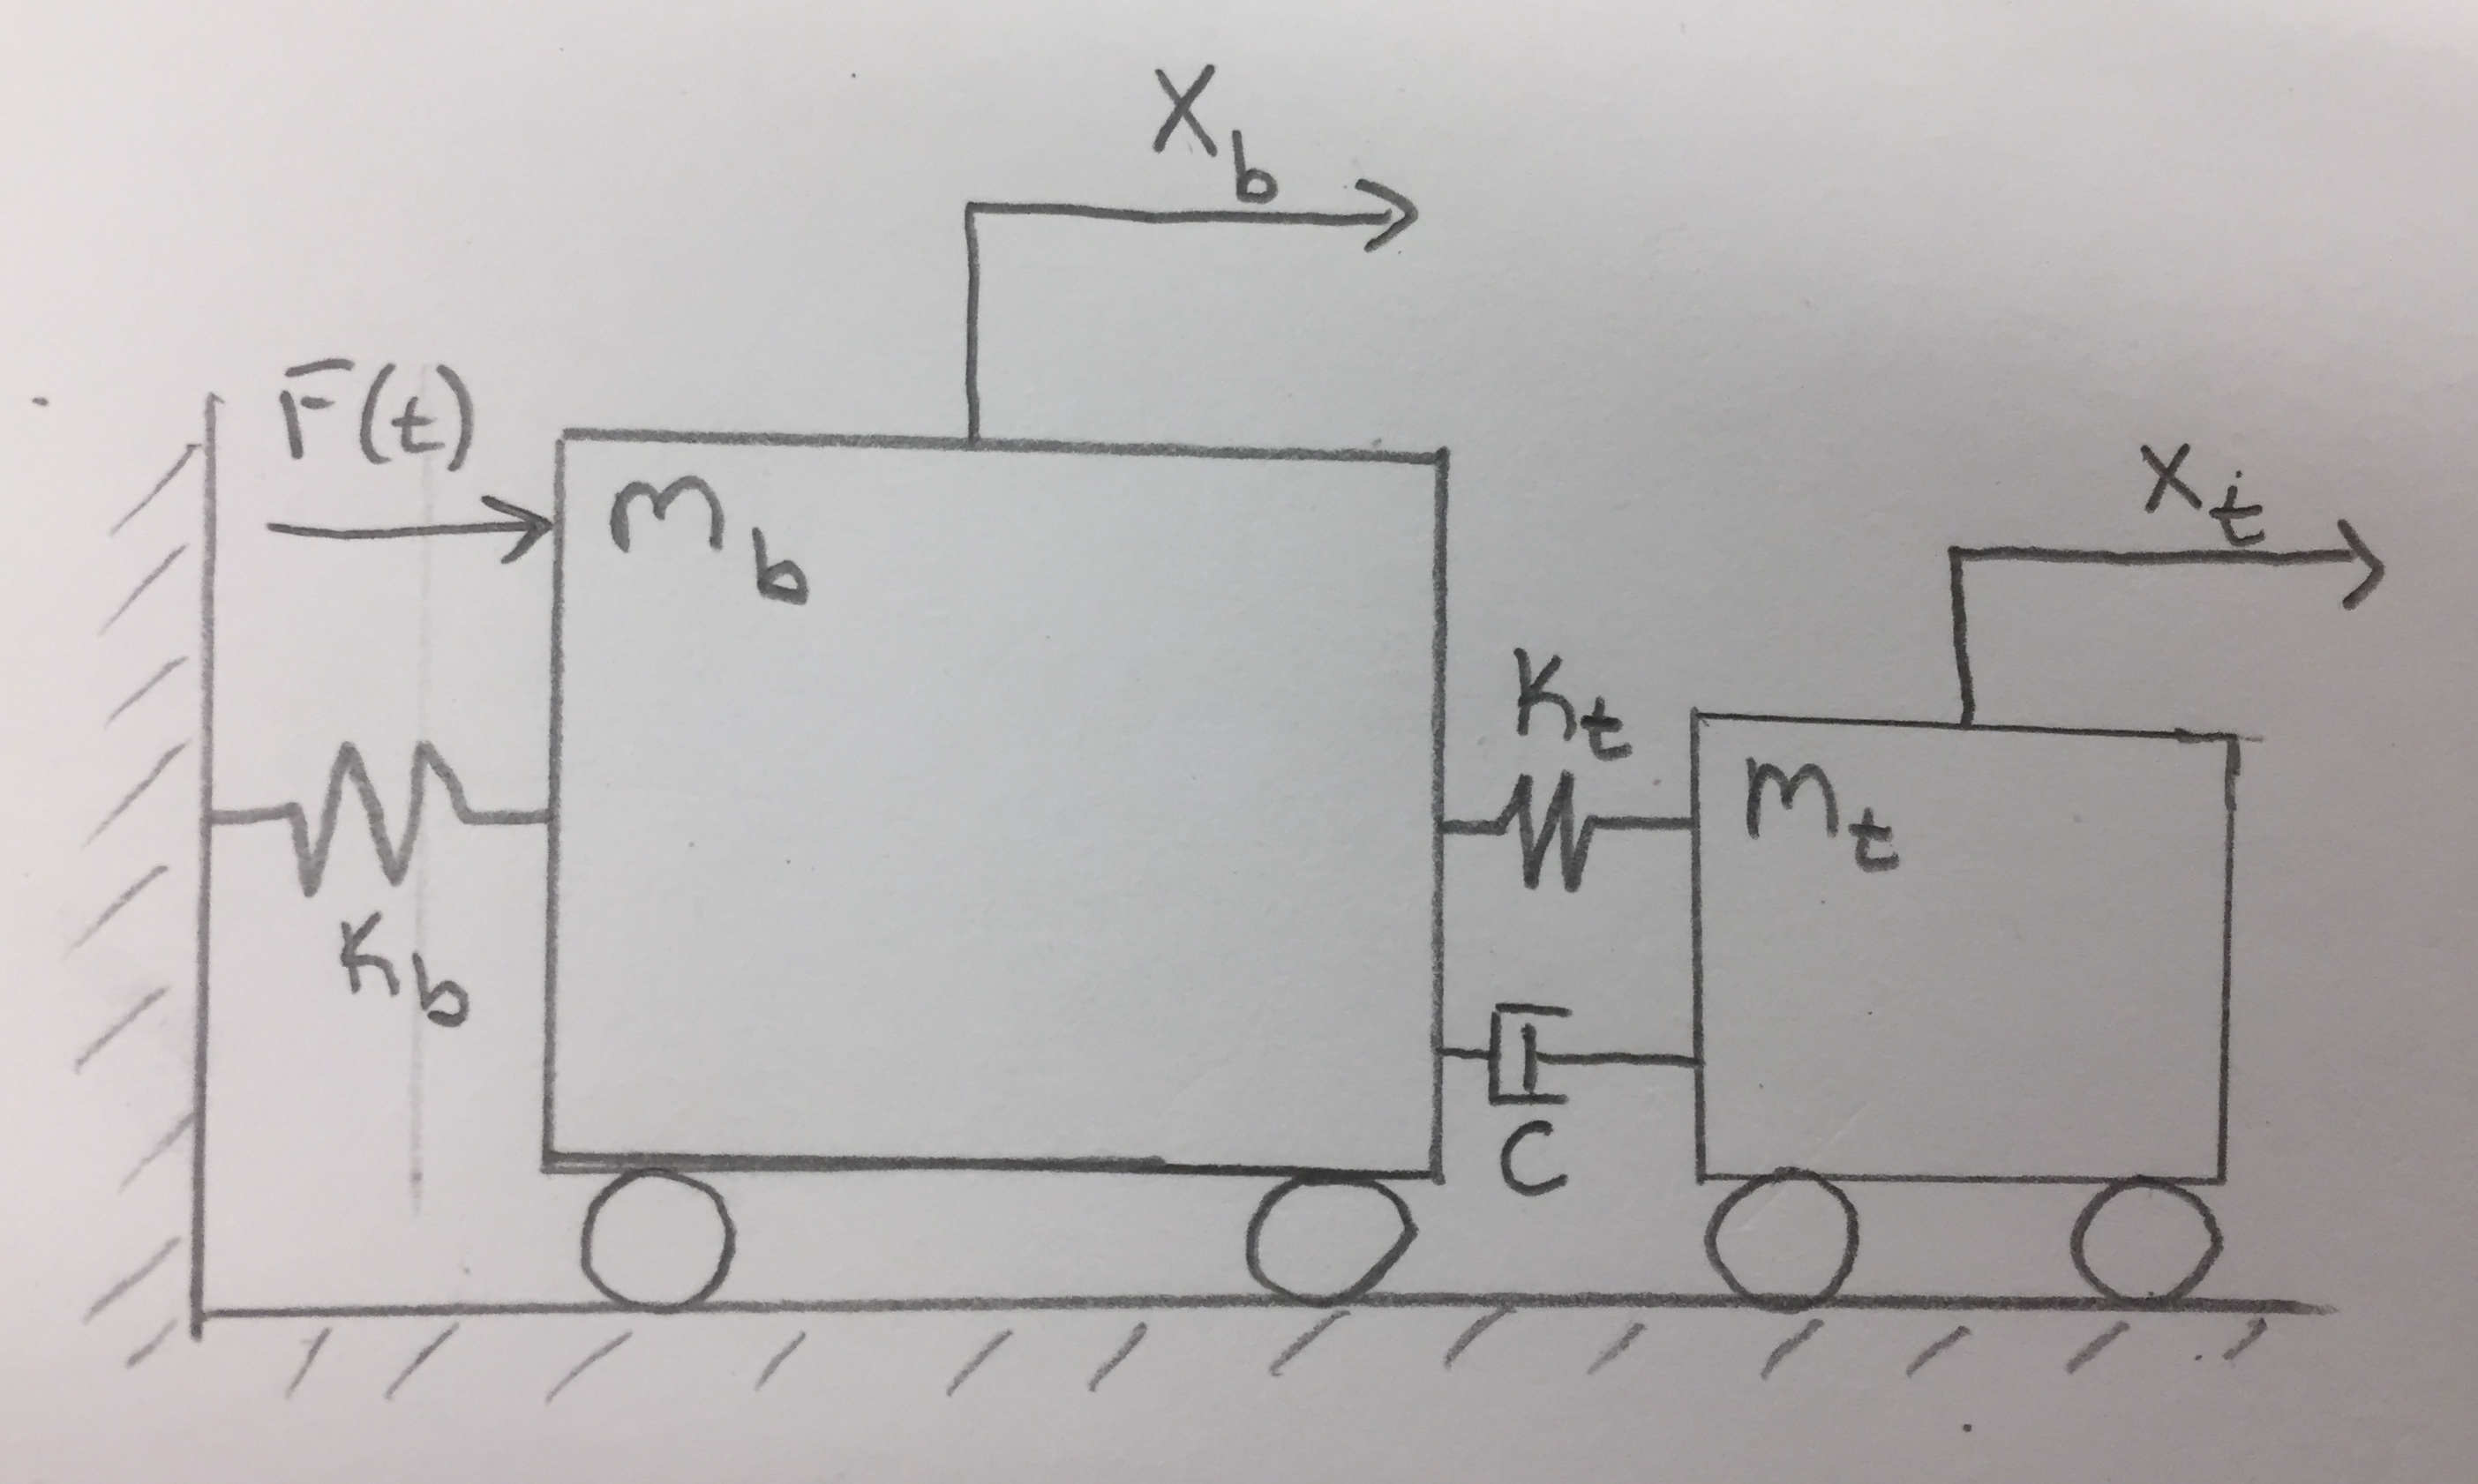
\includegraphics[width=0.45\textwidth]{figures/IMG_4477.jpg} 
\caption{The system that models the Taipei 101 tower in a SDOF}
\end{figure}
\newpage
This gives rise to the following equations: 

\begin{equation}
m_b \ddot{x_b} + k_b x_b + c \left(\dot{x_b} - \dot{x_t}\right) + k_t \left({x_b} - {x_t}\right) = F(t) 
\label{RP1}
\end{equation}

\begin{equation}
m_t \ddot{x_t} + c \left(\dot{x_t} - \dot{x_b}\right) + k_t \left({x_t} - {x_b}\right) = 0
\label{RP2}
\end{equation}
\newline

Equation \ref{RP1} was derived from the free-body diagram for the forces acting on $m_b$ and Equation \ref{RP2} was derived from the free-body diagram for the forces acting on $m_t$. 
\newline

The initial conditions were assumed to be $x_b = 0$ and $x_t = 0$, as well as all the respective derivatives, for $t = 0$, for the purpose of this model.
\newline

The variables and constants used in these equations are defined as follows: 
\begin{itemize}
  \item Mass of the TMD = $m_t=660,000$ kg
  \item Mass of the Building = $m_b = 700000000$ kg
  \item Horizontal movement of Building = $ x_b $, in meters
  \item Horizontal movement of TMD = $ x_t $, in meters
  \item Spring constant of Building = $k_b = 3.69 * 10^9 \: \frac{N}{m} $
  \item Spring constant of TMD = $k_t = 525399.6 \: \frac{N}{m}$
  \item Damping constant = $c = 55353.5 \: \frac{Ns}{m}$
  \item Forcing function = $F(t) = 33064704 $, in Newtons
\end{itemize}

\section*{Assumptions}
\begin{itemize}
	\item The worst case scenario for the building would occur if the the external forces act in resonance with the building's natural frequency. 
    \item If the force matches the buildings resonance frequency, the maximum force can be considered constant. 
    \item The maximum amplitude of the TMD can be derived from the maximum force caused by a typhoon strength wind on the building.
	\item The building's face can be approximated as a rectangle that is 50m wide and 508 m tall[1].
	\item The TMD can be treated as a solid sphere with radius 5.5m rather than layers of plates.
    \item The building's spring coefficient can be derived from the properties of the concrete mega-pillars, which can be approximated as one pillar with the same area as 8 of the pillars together.
    \item The viscous dampers act with a single degree of freedom and apply force only in the horizontal direction.
    \item The 8 42m length cables that hold up the TMD wrap underneath the sphere and back up again, suspending it at a height of 12.36m below the 91st floor.
    \item Assume the vertical motion of the TMD is negligible, therefore it can be modeled as a spring, as opposed to a pendulum.
    \item The internal dampening of the building is negligible in comparison to dampening caused by the suspended mass.  
    \item Assume that the largest applied force will be caused by typhoon strength winds acting on a building as opposed to the oscillatory force applied by an earthquake.
\end{itemize}


\section*{Calculations}
$k_t$ was derived through the spring coefficient formula $ F = -kx $ with trigonometry used to obtain the force in the x direction and 1.5m used as the max x distance. $k_b$ was derived from the stress-strain equation and the spring formula to get $k = \frac{YA}{L}$, where Y is the Young's modulus of the concrete pillars, A is the cross-sectional area affected by shear and L is the length of the pillar. c was derived from the formula $c = 2\zeta\sqrt[]{km}$, with zeta being 4.7$\%$ [6], with k and m being the stiffness and the mass of the TMD, respectively.
\newline
Equation \ref{RP3} was derived using Gaussian elimination on Equation \ref{RP1} and Equation \ref{RP2} to eliminate the variable $x_b$ resulting in a fourth order linear ODE.

\begin{equation}
m_b m_t \frac{d^4x_t}{dt^4} + (m_b+m_t)c\frac{d^3x_t}{dt^3} + (m_b k_t+m_t k_b+m_t k_t)\frac{d^2x_t}{dt^2} + ck_b\frac{dx_t}{dt}+k_bk_t = c\frac{dF(t)}{dt}+k_tF(t)
\label{RP3}
\end{equation}

Equation \ref{RP3} was solved using software on wolfram-alpha with the known constants plugged into their respective places to produce the general solution in Equation 4:
\newline
\begin{center}
$x_t = c_1 e^{-0.0419187t} sin(0.891162 t) + c_3 e^{-0.0000553153 t} sin(2.29614 t)$ \newline $+ c_2 e^{-0.0419187 t} cos(0.891162 t) + c_4 e^{-0.0000553153 t} cos(2.29614 t) + 0.0111735$ \qquad \qquad \ (4)
\end{center}

Using the initial conditions the following integrative constants were obtained:
\begin{itemize}
\item $c_1$ = -0.0318
\item $c_2$ = -1.3422
\item $c_3$ = 0.0028
\item $c_4$ = 0.00065
\end{itemize}

\section*{Analysis}
\subsection*{Max Amplitude}
The forcing function $F(t)$ is the force being applied to the structure that acts in the x direction only (SDOF system).

For the force of wind acting on the building we have: $F_W = \frac{1}{2} \rho V^2 A$, with $\rho$ being the density of air (1.13$\frac{kg}{m^3}$)[5], V being the average wind speed during a typhoon (48 $\frac{m}{s}$)[8], and A being the area that the wind is pushing on. This results in a force of $3.3*10^7$ Newtons being applied to the building during a typhoon. With this constant force in our differential equation, the maximum amplitude was obtained using Desmos graphing technology, the function for $x_t(t)$ was graphed and a value of 1.331m was obtained as a maximum amplitude for the displacement of the mass.

The damping followed an exponential decay that is shown in (Figure 3), and took a reasonable amount of time to settle into low amplitude oscillation patterns (approx. 10cm at 60 seconds and $<$1 cm at 120 seconds).

\begin{figure}[h!]
\centering
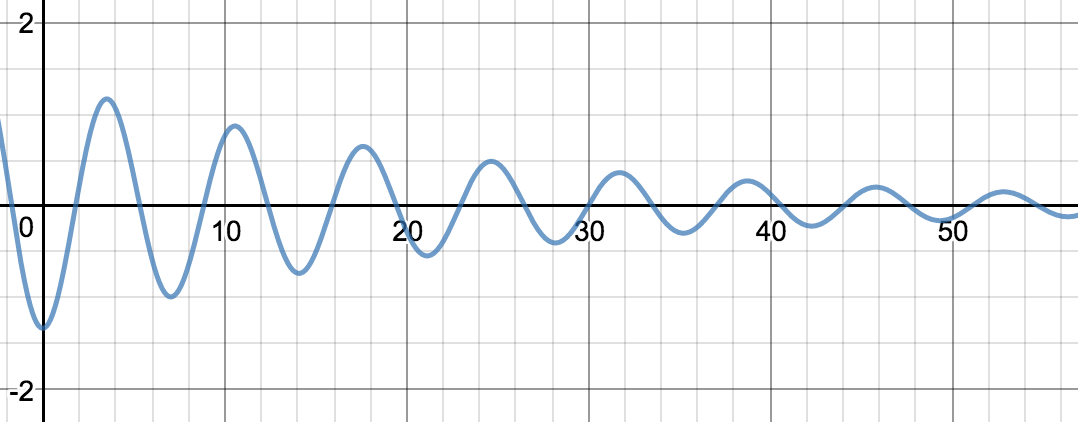
\includegraphics[width=0.45\textwidth]{figures/graph.png} 
\caption{The graph of motion in the x direction of the TMD}
\end{figure}

\section*{Conclusion}
In order to simplify the Taipei 101 it was treated as a SDOF system. The mass of the building and the mass of the tuned mass damper caused the  lateral movement of the building to be dampened as the TMD oscillates as shown in (Figure 3). The maximum amplitude of 1.311m fell within the allowable range of 1.5m, which means the model used was not unrealistic.


\newpage
\section*{Students' contributions}
John and David worked together to understand the problem and write the numerical codes. The assumptions were brainstormed by both David and John. The summary of the problem and assumptions were written by John and the equations and calculations were derived by David. Both students corrected the final report.

\section*{References}

\begin{list}{}{%
\setlength{\topsep}{0pt}%
\setlength{\leftmargin}{0.3in}%
\setlength{\listparindent}{-0.3in}%
\setlength{\itemindent}{-0.3in}%
\setlength{\parsep}{\parskip}%
}%
\item[]
[1] Archinomy.com. (2017). Taipei 101 - A case-study | Archinomy. [online] Available at: http://www.archinomy.com/case-studies/671/taipei-101-a-case-study [Accessed 28 Nov. 2017].
\item[]
[2] Ching-Chang, C. (2017). Structural Design of Taipei 101 Tower. [ebook] 
Available at: http://conf.ncree.org.tw/download%5Ci0981026-structural%20design%20of%20taipei%20101%20tower.pdf 
[Accessed 29 Nov. 2017].
\item[]
[3] Desmos Graphing Calculator. (2017). Desmos | Graphing Calculator. [online] Available at: https://www.desmos.com/calculator [Accessed 1 Dec. 2017].
\item[]
[4] Effa, D. and Lambert, S. (2017). Taipei 101 Tuned Mass Damper Analysis. [ebook] Available at: \url{https://learn.uwaterloo.ca/d2l/le/content/336286/viewContent/1989179/View?ou=336286} [Accessed 28 Nov. 2017].
\item[]
[5] \url{Engineeringtoolbox.com}. (2017). Air - Altitude, Density and Specific Volume. [online] Available at: \url{https://www.engineeringtoolbox.com/air-altitude-density}
\newline
\url{-volume-d_195.html} [Accessed 1 Dec. 2017].
\item[]
[6] Kourakis, I. (2007). Structural systems and tuned mass dampers of super-tall buildings : case study of Taipei 101. [ebook] Massachusetts Institute of Technology. Available at: https://dspace.mit.edu/handle/1721.1/38947 [Accessed 28 Nov. 2017].
\item[]
[7] Rana, R. (2017). Response Control of Structures by Tuned Mass Dampers and their Generalizations. [ebook] Buffalo. Available at: \url{http://www.iitk.ac.in/nicee/wcee/article/11_498.PDF} [Accessed 28 Nov. 2017].
\item[]
[8] Tuan, A. and Shang, G. (2017). Vibration Control in a 101-Storey Building Using a Tuned Mass Damper. [ebook] Available at: \url{https://pdfs.semanticscholar.org/996c/ad4e06286d61eacb5c739be697a690c11dd3.pdf} [Accessed 29 Nov. 2017].
\item[]
[9] Wolframalpha.com. (2017). Wolfram|Alpha: Making the world’s knowledge computable. [online] Available at: https://www.wolframalpha.com [Accessed 30 Nov. 2017].

\end{list}
\end{document}
%%% Local Variables: 
%%% mode: latex
%%% TeX-master: t
%%% End: 
